\documentclass{IEEEtran}

\usepackage[utf8]{inputenc}
\usepackage[english]{babel}
\usepackage{graphicx}
\usepackage{url}
%\usepackage[margin = 1in]{geometry}
 
\usepackage{biblatex}
\addbibresource{sources.bib}

\title{ET4394 Wireless Networking - Decoding RFD900 packets}
\date{\today}
\author{
Bart Rijnders - 4103505 \\
Bernard Bekker - 4221656 
}

\begin{document}

\maketitle

\begin{abstract}

This report describes a method to decode packets from the RFD900 900MHz Ultra Long Range Radio Modem using MATLAB. A script was written that is able to demodulate and decode a signal from the modem that was captured using an SDR. The script outputs an array of bytes that represent a packet sent by the modem. Finally the script is also able to do a checksum of the packet using a 16 bit CRC that was ported to matlab from the firmware of the device.

\end{abstract}

\section{Introduction}

The RFD900 is an Ultra Long Range Radio Modem that operates on a frequency of 900MHz, has a transmit power of 1 Watt and an advertised range of 40 kilometers. It uses FSK modulation, data whitening before transmitting and FHSS to switch carrier frequency after a packet has been transmitted. These options make decoding the signal a challenging task. It also offers options such as AES encryption which has been turned off for this project. The firmware of the RFD900 is open source and can be found on GitHub \cite{4509719}.

\section{Methodology}

\subsection{Data Capture}

Data was captured by using an SDR near the RFD900 modem transmitting random data. This resulted in a raw IQ data file which was cut using Audacity to isolate a transmission of two packets in succession. This was done for simplicity to not have to process a large signal. A graph of the resulting signal can be seen in figure \ref{fig:2_packets_sig}. It can be seen that during the preamble the amplitude slowly increases to it's peak values.

\begin{figure}[h]
		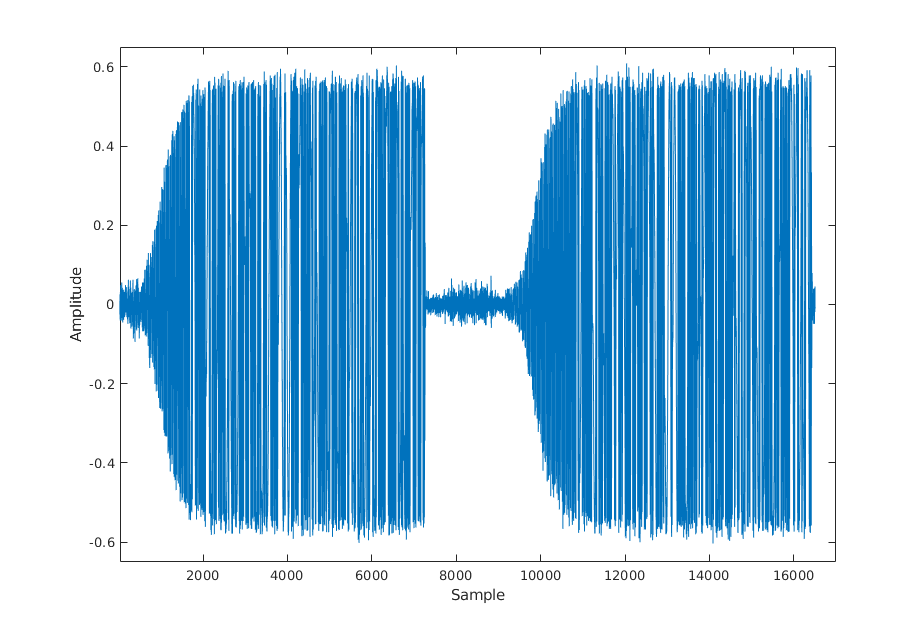
\includegraphics[width=0.5\textwidth]{plots/Two_packets_signal.png}
		\caption{Signal of two subsequently received packets}
		\label{fig:2_packets_sig}
\end{figure}



\subsection{Script}

The first attempt to decode a packet was done using GNU Radio, however since the options for clock recovery in GNU Radio are limited and not well documented a switch was made to MATLAB instead. 

In MATLAB the script consists of multiple separate functions, see the full script for details. First the data file is read and the IQ values are represented as a vector with imaginary numbers. Then a threshold is used to determine where a packet starts and ends, to filter out noise. This is done by creating a mask of logical values indicating whether a data signal is present at a given index of the vector. It can be used to isolate the two different packets that have been transmitted. This mask is then applied to the original signal to obtain the two different packets as vectors.  

These two isolated signals are then decoded by a separate function. Firstly the signal is tuned have the signal centered around zero. %rephrase to correct words
This is done by first determining the mean frequency of the signal which can be easily done using an existing function in MATLAB. This mean frequency can be seen as the offset. Then each sample of the signal is multiplied by the offset to obtain a signal centered around 0 Hz. The signal is then run through a fourth order butterworth filter and downsampled.

After the signal has been centered, filtered and downsampled it is converted to a sequence of bits. This is done by first determining the positions of the signal where it crosses the x-axis, meaning the signal is equal to zero. %rephrase with units
To determine if a bit should be one or zero the length between two successive crossings is measured and divided by. %insert correct unit here

This results in a stream of bits which can be parsed by first finding the preamble. The preamble mask used is an alternating 24 bit array of ones and zeros starting with a zero. It will occur only once per packet, so it is used to determine the start of the data. Besides a preamble a syncword is used to find the start of a header. 

(Insert data dewhitening here).

Finally a CRC check of the packet can be done, this code is ported directly from the firmware to matlab to make sure the check is correct. It uses a lookup table instead of actually doing the calculations required. This is done to save time, in our case however this is not important since the signal is not decoded in real-time.

\section{Results}

\begin{table}[h]
\centering
\caption{Decoded Packet}
\label{tbl1}
\begin{tabular}{lll}
Byte & Meaning & Binary Value \\
\hline
0       & 98                          & 10000001  \\
1       & 52                          & 00011111  \\
2       & 67                          & 10000000   \\
3       & 100                         & 10000001    \\
4      & CRC fields                   & 00000000 \\
5      & CRC fields                   & 00000000 \\
6      & CRC fields                   & 00000000 \\
7      & CRC fields                   & 11001111 \\
8      & CRC fields                   & 11111111 \\
9      & CRC fields                   & 11101010 \\
10      & CRC fields                  & 11111111 \\
11     & CRC fields                   & 11001110 \\
12     & CRC fields                   & 00000000 \\
13     & CRC fields                   & 11001111 \\
14     & CRC fields                   & 00000000 \\
15     & CRC fields                   & 00000000 \\
16     & CRC fields                   & 00000000 \\
17     & CRC fields                   & 11001110 \\
18     & CRC fields                   & 00000000 \\
19     & CRC fields                   & 10000010 \\
20     & CRC fields                   & 11110111 \\
21     & 8 bit CRC high value       & 01011111 \\
22     & 8 bit CRC low value        & 10001001 \\
\end{tabular}
\end{table}

\section{Discussion}

A valuable addition to the current system would be to enable it to decode a signal in real-time. This can be done by outputting the data over a virtual COM port or a TCP port, which can be connected to an existing telemetry application used by Formula Student Team Delft. This application uses a graphical user interface to display all the received data.
\printbibliography

\end{document}